% Options for packages loaded elsewhere
\PassOptionsToPackage{unicode}{hyperref}
\PassOptionsToPackage{hyphens}{url}
\PassOptionsToPackage{dvipsnames,svgnames,x11names}{xcolor}
%
\documentclass[
  12pt,
  letterpaper,
  DIV=11,
  numbers=noendperiod]{scrartcl}

\usepackage{amsmath,amssymb}
\usepackage{lmodern}
\usepackage{iftex}
\ifPDFTeX
  \usepackage[T1]{fontenc}
  \usepackage[utf8]{inputenc}
  \usepackage{textcomp} % provide euro and other symbols
\else % if luatex or xetex
  \usepackage{unicode-math}
  \defaultfontfeatures{Scale=MatchLowercase}
  \defaultfontfeatures[\rmfamily]{Ligatures=TeX,Scale=1}
  \setmainfont[]{Verdana}
\fi
% Use upquote if available, for straight quotes in verbatim environments
\IfFileExists{upquote.sty}{\usepackage{upquote}}{}
\IfFileExists{microtype.sty}{% use microtype if available
  \usepackage[]{microtype}
  \UseMicrotypeSet[protrusion]{basicmath} % disable protrusion for tt fonts
}{}
\makeatletter
\@ifundefined{KOMAClassName}{% if non-KOMA class
  \IfFileExists{parskip.sty}{%
    \usepackage{parskip}
  }{% else
    \setlength{\parindent}{0pt}
    \setlength{\parskip}{6pt plus 2pt minus 1pt}}
}{% if KOMA class
  \KOMAoptions{parskip=half}}
\makeatother
\usepackage{xcolor}
\setlength{\emergencystretch}{3em} % prevent overfull lines
\setcounter{secnumdepth}{-\maxdimen} % remove section numbering
% Make \paragraph and \subparagraph free-standing
\ifx\paragraph\undefined\else
  \let\oldparagraph\paragraph
  \renewcommand{\paragraph}[1]{\oldparagraph{#1}\mbox{}}
\fi
\ifx\subparagraph\undefined\else
  \let\oldsubparagraph\subparagraph
  \renewcommand{\subparagraph}[1]{\oldsubparagraph{#1}\mbox{}}
\fi

\usepackage{color}
\usepackage{fancyvrb}
\newcommand{\VerbBar}{|}
\newcommand{\VERB}{\Verb[commandchars=\\\{\}]}
\DefineVerbatimEnvironment{Highlighting}{Verbatim}{commandchars=\\\{\}}
% Add ',fontsize=\small' for more characters per line
\usepackage{framed}
\definecolor{shadecolor}{RGB}{241,243,245}
\newenvironment{Shaded}{\begin{snugshade}}{\end{snugshade}}
\newcommand{\AlertTok}[1]{\textcolor[rgb]{0.68,0.00,0.00}{#1}}
\newcommand{\AnnotationTok}[1]{\textcolor[rgb]{0.37,0.37,0.37}{#1}}
\newcommand{\AttributeTok}[1]{\textcolor[rgb]{0.40,0.45,0.13}{#1}}
\newcommand{\BaseNTok}[1]{\textcolor[rgb]{0.68,0.00,0.00}{#1}}
\newcommand{\BuiltInTok}[1]{\textcolor[rgb]{0.00,0.23,0.31}{#1}}
\newcommand{\CharTok}[1]{\textcolor[rgb]{0.13,0.47,0.30}{#1}}
\newcommand{\CommentTok}[1]{\textcolor[rgb]{0.37,0.37,0.37}{#1}}
\newcommand{\CommentVarTok}[1]{\textcolor[rgb]{0.37,0.37,0.37}{\textit{#1}}}
\newcommand{\ConstantTok}[1]{\textcolor[rgb]{0.56,0.35,0.01}{#1}}
\newcommand{\ControlFlowTok}[1]{\textcolor[rgb]{0.00,0.23,0.31}{#1}}
\newcommand{\DataTypeTok}[1]{\textcolor[rgb]{0.68,0.00,0.00}{#1}}
\newcommand{\DecValTok}[1]{\textcolor[rgb]{0.68,0.00,0.00}{#1}}
\newcommand{\DocumentationTok}[1]{\textcolor[rgb]{0.37,0.37,0.37}{\textit{#1}}}
\newcommand{\ErrorTok}[1]{\textcolor[rgb]{0.68,0.00,0.00}{#1}}
\newcommand{\ExtensionTok}[1]{\textcolor[rgb]{0.00,0.23,0.31}{#1}}
\newcommand{\FloatTok}[1]{\textcolor[rgb]{0.68,0.00,0.00}{#1}}
\newcommand{\FunctionTok}[1]{\textcolor[rgb]{0.28,0.35,0.67}{#1}}
\newcommand{\ImportTok}[1]{\textcolor[rgb]{0.00,0.46,0.62}{#1}}
\newcommand{\InformationTok}[1]{\textcolor[rgb]{0.37,0.37,0.37}{#1}}
\newcommand{\KeywordTok}[1]{\textcolor[rgb]{0.00,0.23,0.31}{#1}}
\newcommand{\NormalTok}[1]{\textcolor[rgb]{0.00,0.23,0.31}{#1}}
\newcommand{\OperatorTok}[1]{\textcolor[rgb]{0.37,0.37,0.37}{#1}}
\newcommand{\OtherTok}[1]{\textcolor[rgb]{0.00,0.23,0.31}{#1}}
\newcommand{\PreprocessorTok}[1]{\textcolor[rgb]{0.68,0.00,0.00}{#1}}
\newcommand{\RegionMarkerTok}[1]{\textcolor[rgb]{0.00,0.23,0.31}{#1}}
\newcommand{\SpecialCharTok}[1]{\textcolor[rgb]{0.37,0.37,0.37}{#1}}
\newcommand{\SpecialStringTok}[1]{\textcolor[rgb]{0.13,0.47,0.30}{#1}}
\newcommand{\StringTok}[1]{\textcolor[rgb]{0.13,0.47,0.30}{#1}}
\newcommand{\VariableTok}[1]{\textcolor[rgb]{0.07,0.07,0.07}{#1}}
\newcommand{\VerbatimStringTok}[1]{\textcolor[rgb]{0.13,0.47,0.30}{#1}}
\newcommand{\WarningTok}[1]{\textcolor[rgb]{0.37,0.37,0.37}{\textit{#1}}}

\providecommand{\tightlist}{%
  \setlength{\itemsep}{0pt}\setlength{\parskip}{0pt}}\usepackage{longtable,booktabs,array}
\usepackage{calc} % for calculating minipage widths
% Correct order of tables after \paragraph or \subparagraph
\usepackage{etoolbox}
\makeatletter
\patchcmd\longtable{\par}{\if@noskipsec\mbox{}\fi\par}{}{}
\makeatother
% Allow footnotes in longtable head/foot
\IfFileExists{footnotehyper.sty}{\usepackage{footnotehyper}}{\usepackage{footnote}}
\makesavenoteenv{longtable}
\usepackage{graphicx}
\makeatletter
\def\maxwidth{\ifdim\Gin@nat@width>\linewidth\linewidth\else\Gin@nat@width\fi}
\def\maxheight{\ifdim\Gin@nat@height>\textheight\textheight\else\Gin@nat@height\fi}
\makeatother
% Scale images if necessary, so that they will not overflow the page
% margins by default, and it is still possible to overwrite the defaults
% using explicit options in \includegraphics[width, height, ...]{}
\setkeys{Gin}{width=\maxwidth,height=\maxheight,keepaspectratio}
% Set default figure placement to htbp
\makeatletter
\def\fps@figure{htbp}
\makeatother

<script src="Fiber_analysis_quarto_files/libs/htmlwidgets-1.5.4/htmlwidgets.js"></script>
<link href="Fiber_analysis_quarto_files/libs/datatables-css-0.0.0/datatables-crosstalk.css" rel="stylesheet" />
<script src="Fiber_analysis_quarto_files/libs/datatables-binding-0.26/datatables.js"></script>
<script src="Fiber_analysis_quarto_files/libs/jquery-3.6.0/jquery-3.6.0.min.js"></script>
<link href="Fiber_analysis_quarto_files/libs/dt-core-1.12.1/css/jquery.dataTables.min.css" rel="stylesheet" />
<link href="Fiber_analysis_quarto_files/libs/dt-core-1.12.1/css/jquery.dataTables.extra.css" rel="stylesheet" />
<script src="Fiber_analysis_quarto_files/libs/dt-core-1.12.1/js/jquery.dataTables.min.js"></script>
<script src="Fiber_analysis_quarto_files/libs/jszip-1.12.1/jszip.min.js"></script>
<script src="Fiber_analysis_quarto_files/libs/pdfmake-1.12.1/pdfmake.js"></script>
<script src="Fiber_analysis_quarto_files/libs/pdfmake-1.12.1/vfs_fonts.js"></script>
<link href="Fiber_analysis_quarto_files/libs/dt-ext-buttons-1.12.1/css/buttons.dataTables.min.css" rel="stylesheet" />
<script src="Fiber_analysis_quarto_files/libs/dt-ext-buttons-1.12.1/js/dataTables.buttons.min.js"></script>
<script src="Fiber_analysis_quarto_files/libs/dt-ext-buttons-1.12.1/js/buttons.html5.min.js"></script>
<script src="Fiber_analysis_quarto_files/libs/dt-ext-buttons-1.12.1/js/buttons.colVis.min.js"></script>
<script src="Fiber_analysis_quarto_files/libs/dt-ext-buttons-1.12.1/js/buttons.print.min.js"></script>
<link href="Fiber_analysis_quarto_files/libs/crosstalk-1.2.0/css/crosstalk.min.css" rel="stylesheet" />
<script src="Fiber_analysis_quarto_files/libs/crosstalk-1.2.0/js/crosstalk.min.js"></script>
\KOMAoption{captions}{tableheading}
\makeatletter
\makeatother
\makeatletter
\makeatother
\makeatletter
\@ifpackageloaded{caption}{}{\usepackage{caption}}
\AtBeginDocument{%
\ifdefined\contentsname
  \renewcommand*\contentsname{Table of contents}
\else
  \newcommand\contentsname{Table of contents}
\fi
\ifdefined\listfigurename
  \renewcommand*\listfigurename{List of Figures}
\else
  \newcommand\listfigurename{List of Figures}
\fi
\ifdefined\listtablename
  \renewcommand*\listtablename{List of Tables}
\else
  \newcommand\listtablename{List of Tables}
\fi
\ifdefined\figurename
  \renewcommand*\figurename{Figure}
\else
  \newcommand\figurename{Figure}
\fi
\ifdefined\tablename
  \renewcommand*\tablename{Table}
\else
  \newcommand\tablename{Table}
\fi
}
\@ifpackageloaded{float}{}{\usepackage{float}}
\floatstyle{ruled}
\@ifundefined{c@chapter}{\newfloat{codelisting}{h}{lop}}{\newfloat{codelisting}{h}{lop}[chapter]}
\floatname{codelisting}{Listing}
\newcommand*\listoflistings{\listof{codelisting}{List of Listings}}
\makeatother
\makeatletter
\@ifpackageloaded{caption}{}{\usepackage{caption}}
\@ifpackageloaded{subcaption}{}{\usepackage{subcaption}}
\makeatother
\makeatletter
\@ifpackageloaded{tcolorbox}{}{\usepackage[many]{tcolorbox}}
\makeatother
\makeatletter
\@ifundefined{shadecolor}{\definecolor{shadecolor}{rgb}{.97, .97, .97}}
\makeatother
\makeatletter
\makeatother
\ifLuaTeX
  \usepackage{selnolig}  % disable illegal ligatures
\fi
\IfFileExists{bookmark.sty}{\usepackage{bookmark}}{\usepackage{hyperref}}
\IfFileExists{xurl.sty}{\usepackage{xurl}}{} % add URL line breaks if available
\urlstyle{same} % disable monospaced font for URLs
\hypersetup{
  pdftitle={Tph2 Fiber Analysis},
  colorlinks=true,
  linkcolor={blue},
  filecolor={Maroon},
  citecolor={Blue},
  urlcolor={Blue},
  pdfcreator={LaTeX via pandoc}}

\title{Tph2 Fiber Analysis}
\author{}
\date{}

\begin{document}
\maketitle
\ifdefined\Shaded\renewenvironment{Shaded}{\begin{tcolorbox}[interior hidden, borderline west={3pt}{0pt}{shadecolor}, frame hidden, breakable, boxrule=0pt, enhanced, sharp corners]}{\end{tcolorbox}}\fi

\hypertarget{introduction}{%
\subsection{Introduction}\label{introduction}}

This notebook takes in exported CellProfiler data along with a metadata
table with information about treatment for each mouse and outputs graphs
and statistics about the fibers.

\hypertarget{setup}{%
\subsection{Setup}\label{setup}}

\begin{Shaded}
\begin{Highlighting}[]
\FunctionTok{library}\NormalTok{(ggplot2)}
\end{Highlighting}
\end{Shaded}

\begin{verbatim}
Warning: package 'ggplot2' was built under R version 4.1.2
\end{verbatim}

\begin{Shaded}
\begin{Highlighting}[]
\FunctionTok{library}\NormalTok{(here)}
\end{Highlighting}
\end{Shaded}

\begin{verbatim}
here() starts at /Users/rsenft/Documents/GitHub/RebeccaSenft_Projects/002_Dymecki_neuro/Batch_3_fibers/Fibers_analysis
\end{verbatim}

\begin{Shaded}
\begin{Highlighting}[]
\FunctionTok{library}\NormalTok{(dplyr)}
\end{Highlighting}
\end{Shaded}

\begin{verbatim}
Warning: package 'dplyr' was built under R version 4.1.2
\end{verbatim}

\begin{verbatim}

Attaching package: 'dplyr'
\end{verbatim}

\begin{verbatim}
The following objects are masked from 'package:stats':

    filter, lag
\end{verbatim}

\begin{verbatim}
The following objects are masked from 'package:base':

    intersect, setdiff, setequal, union
\end{verbatim}

\begin{Shaded}
\begin{Highlighting}[]
\FunctionTok{library}\NormalTok{(RColorBrewer)}
\end{Highlighting}
\end{Shaded}

\begin{verbatim}
Warning: package 'RColorBrewer' was built under R version 4.1.2
\end{verbatim}

\begin{Shaded}
\begin{Highlighting}[]
\FunctionTok{library}\NormalTok{(readr)}
\end{Highlighting}
\end{Shaded}

\begin{verbatim}
Warning: package 'readr' was built under R version 4.1.2
\end{verbatim}

\begin{Shaded}
\begin{Highlighting}[]
\FunctionTok{library}\NormalTok{(DT)}
\end{Highlighting}
\end{Shaded}

\begin{verbatim}
Warning: package 'DT' was built under R version 4.1.2
\end{verbatim}

\hypertarget{get-data}{%
\subsection{Get data}\label{get-data}}

Note that the CSV had to be corrected because there is one filename with
ROB instead of ROb and because not all the metadata is extracted
correctly (inconsistent filenames), so I manually corrected this in
Excel using Flash Fill and correcting the mispelling and saved this as
\texttt{Tph2\_Per\_Image\_metadata\_corrected.csv}.

\begin{Shaded}
\begin{Highlighting}[]
\NormalTok{path\_to\_csv\_folder }\OtherTok{=} \FunctionTok{here}\NormalTok{(}\StringTok{"csvs"}\NormalTok{)}
\NormalTok{save\_path }\OtherTok{\textless{}{-}}\NormalTok{ path\_to\_csv\_folder}
\NormalTok{img\_filename}\OtherTok{=}\StringTok{"Tph2\_Per\_Image\_metadata\_corrected.csv"}
\NormalTok{sc\_filename}\OtherTok{=}\StringTok{"Tph2\_Per\_BorderedCells.csv"}

\NormalTok{metadata\_filename}\OtherTok{=}\StringTok{"Litter{-}groups{-}A{-}through{-}ii.csv"} \CommentTok{\#note I gave this headings}

\CommentTok{\#load data and metadata for images}
\NormalTok{image\_df }\OtherTok{\textless{}{-}} \FunctionTok{read.csv}\NormalTok{(}\FunctionTok{here}\NormalTok{(path\_to\_csv\_folder,img\_filename), }\AttributeTok{check.names=}\ConstantTok{FALSE}\NormalTok{)}
\NormalTok{metadata }\OtherTok{\textless{}{-}} \FunctionTok{read.csv}\NormalTok{(}\FunctionTok{here}\NormalTok{(path\_to\_csv\_folder,metadata\_filename), }\AttributeTok{check.names =} \ConstantTok{FALSE}\NormalTok{)}
\NormalTok{image\_df\_combined }\OtherTok{\textless{}{-}} \FunctionTok{merge}\NormalTok{(image\_df, metadata, }\AttributeTok{by.x=}\StringTok{"Image\_Metadata\_Litter"}\NormalTok{, }\AttributeTok{by.y=}\StringTok{"Litter"}\NormalTok{)}

\CommentTok{\#load data for single cells}
\NormalTok{sc\_df }\OtherTok{\textless{}{-}} \FunctionTok{read.csv}\NormalTok{(}\FunctionTok{here}\NormalTok{(path\_to\_csv\_folder,sc\_filename), }\AttributeTok{check.names=}\ConstantTok{FALSE}\NormalTok{)}
\NormalTok{sc\_df\_combined }\OtherTok{\textless{}{-}} \FunctionTok{merge}\NormalTok{(sc\_df, image\_df\_combined, }\AttributeTok{by=}\StringTok{"ImageNumber"}\NormalTok{)}
\end{Highlighting}
\end{Shaded}

We also need to compute the average length of a branch, taken as the
total skeleton length / (number of trunks + number of non-trunk
branches).

\begin{Shaded}
\begin{Highlighting}[]
\NormalTok{sc\_df\_combined }\OtherTok{\textless{}{-}}\NormalTok{ sc\_df\_combined }\SpecialCharTok{\%\textgreater{}\%} 
  \FunctionTok{mutate}\NormalTok{(}\AttributeTok{BorderedCells\_ObjectSkeleton\_avg\_branch\_length =}\NormalTok{ BorderedCells\_ObjectSkeleton\_TotalObjectSkltnLngth\_MrphlgclSkltn}\SpecialCharTok{/}\NormalTok{(BorderedCells\_ObjectSkeleton\_NumberNonTrunkBranchs\_MrphlgclSkltn}\SpecialCharTok{+}\NormalTok{BorderedCells\_ObjectSkeleton\_NumberTrunks\_MorphologicalSkeleton))}
\end{Highlighting}
\end{Shaded}

\hypertarget{summarize-skeleton-features}{%
\subsection{Summarize skeleton
features}\label{summarize-skeleton-features}}

Summarize for each region, mouse, treatment (\texttt{region\_df}) and
for each mouse and treatment group (\texttt{total\_df}).

\begin{Shaded}
\begin{Highlighting}[]
\CommentTok{\# Select only columns with fiber measurements and create summary table:}
\NormalTok{cols2summarize }\OtherTok{\textless{}{-}} \FunctionTok{names}\NormalTok{(sc\_df\_combined)[}\FunctionTok{grepl}\NormalTok{(}\StringTok{"*ObjectSkeleton*"}\NormalTok{, }\FunctionTok{names}\NormalTok{(sc\_df\_combined))] }
\CommentTok{\# make Inf NaN}
\NormalTok{sc\_df\_combined[sc\_df\_combined}\SpecialCharTok{==}\ConstantTok{Inf}\NormalTok{]}\OtherTok{\textless{}{-}} \ConstantTok{NaN}
\CommentTok{\#get morphological skeleton features}

\NormalTok{region\_df }\OtherTok{\textless{}{-}}\NormalTok{ sc\_df\_combined }\SpecialCharTok{\%\textgreater{}\%} 
  \FunctionTok{group\_by}\NormalTok{(ExpGroup, Image\_Metadata\_Mouse, Image\_Metadata\_Region) }\SpecialCharTok{\%\textgreater{}\%}
  \FunctionTok{summarize}\NormalTok{(}\FunctionTok{across}\NormalTok{(}\FunctionTok{all\_of}\NormalTok{(cols2summarize), mean, }\AttributeTok{na.rm=}\ConstantTok{TRUE}\NormalTok{))}
\end{Highlighting}
\end{Shaded}

\begin{verbatim}
`summarise()` has grouped output by 'ExpGroup', 'Image_Metadata_Mouse'. You can
override using the `.groups` argument.
\end{verbatim}

\begin{Shaded}
\begin{Highlighting}[]
\NormalTok{total\_df }\OtherTok{\textless{}{-}}\NormalTok{ region\_df }\SpecialCharTok{\%\textgreater{}\%} 
  \FunctionTok{group\_by}\NormalTok{(ExpGroup, Image\_Metadata\_Mouse) }\SpecialCharTok{\%\textgreater{}\%}
  \FunctionTok{summarize}\NormalTok{(}\FunctionTok{across}\NormalTok{(}\FunctionTok{all\_of}\NormalTok{(cols2summarize), mean, }\AttributeTok{na.rm=}\ConstantTok{TRUE}\NormalTok{))}
\end{Highlighting}
\end{Shaded}

\begin{verbatim}
`summarise()` has grouped output by 'ExpGroup'. You can override using the
`.groups` argument.
\end{verbatim}

\hypertarget{plot-skeleton-features}{%
\subsection{Plot skeleton features}\label{plot-skeleton-features}}

Plot the five features by region and by experimental group
\texttt{ExpGroup}. First, we set up some plotting colors and
descriptions for each variable:

\begin{Shaded}
\begin{Highlighting}[]
\NormalTok{pal}\OtherTok{=}\FunctionTok{c}\NormalTok{(}\StringTok{"\#FFE66D"}\NormalTok{,  }\StringTok{"\#C2CAE8"}\NormalTok{, }\StringTok{"\#FF4365"}\NormalTok{, }\StringTok{"\#00D9C0"}\NormalTok{, }\StringTok{"\#F26419"}\NormalTok{, }\StringTok{"\#86BBD8"}\NormalTok{)}
\NormalTok{pal\_dark}\OtherTok{=}\FunctionTok{c}\NormalTok{(}\StringTok{"\#A38800"}\NormalTok{,  }\StringTok{"\#273568"}\NormalTok{,}\StringTok{"\#FF6B6B"}\NormalTok{, }\StringTok{"\#FF4365"}\NormalTok{, }\StringTok{"\#00D9C0"}\NormalTok{, }\StringTok{"\#F26419"}\NormalTok{, }\StringTok{"\#86BBD8"}\NormalTok{)}

\NormalTok{measurements }\OtherTok{=} \FunctionTok{c}\NormalTok{(}\StringTok{"BorderedCells\_ObjectSkeleton\_NumberBranchEnds\_MorphologicalSkltn"}\NormalTok{, }
                 \StringTok{"BorderedCells\_ObjectSkeleton\_NumberNonTrunkBranchs\_MrphlgclSkltn"}\NormalTok{,}
                 \StringTok{"BorderedCells\_ObjectSkeleton\_NumberTrunks\_MorphologicalSkeleton"}\NormalTok{,}
                 \StringTok{"BorderedCells\_ObjectSkeleton\_TotalObjectSkltnLngth\_MrphlgclSkltn"}\NormalTok{,}
                 \StringTok{"BorderedCells\_ObjectSkeleton\_avg\_branch\_length"}\NormalTok{)}
\NormalTok{desc }\OtherTok{=} \FunctionTok{c}\NormalTok{(}\StringTok{"Number of Branch Termini"}\NormalTok{,}
         \StringTok{"Number of Trunk Branches"}\NormalTok{,}
         \StringTok{"Number of Trunks"}\NormalTok{,}
         \StringTok{"Total Skeleton Length"}\NormalTok{,}
         \StringTok{"Mean Process Length"}\NormalTok{)}
\end{Highlighting}
\end{Shaded}

Here is the function for our box and whisker plot:

\begin{Shaded}
\begin{Highlighting}[]
\NormalTok{plot\_boxwhisker }\OtherTok{\textless{}{-}} \ControlFlowTok{function}\NormalTok{(data, measurements, desc, index, x\_var)\{}
\NormalTok{  meas}\OtherTok{\textless{}{-}}\NormalTok{ measurements[index]}
\NormalTok{  data}\OtherTok{\textless{}{-}}\NormalTok{ data }\SpecialCharTok{\%\textgreater{}\%} \FunctionTok{filter}\NormalTok{(}\FunctionTok{is.finite}\NormalTok{(}\FunctionTok{get}\NormalTok{(meas)))}
\NormalTok{  p }\OtherTok{\textless{}{-}} \FunctionTok{ggplot}\NormalTok{(data, }\FunctionTok{aes}\NormalTok{(}\AttributeTok{x=}\FunctionTok{get}\NormalTok{(x\_var), }\AttributeTok{y=}\FunctionTok{get}\NormalTok{(meas), }\AttributeTok{fill=}\NormalTok{ExpGroup))}\SpecialCharTok{+}
  \FunctionTok{scale\_fill\_manual}\NormalTok{(}\AttributeTok{values=}\NormalTok{pal)}\SpecialCharTok{+}
  \FunctionTok{geom\_boxplot}\NormalTok{(}\AttributeTok{position =} \FunctionTok{position\_dodge}\NormalTok{(}\FloatTok{0.9}\NormalTok{))}\SpecialCharTok{+}
  \FunctionTok{geom\_jitter}\NormalTok{(}\AttributeTok{position =} \FunctionTok{position\_dodge}\NormalTok{(}\FloatTok{0.9}\NormalTok{), }\AttributeTok{alpha=}\FloatTok{0.8}\NormalTok{, }\FunctionTok{aes}\NormalTok{(}\AttributeTok{color=}\NormalTok{ExpGroup))}\SpecialCharTok{+}
  \FunctionTok{scale\_color\_manual}\NormalTok{(}\AttributeTok{values=}\NormalTok{pal\_dark)}\SpecialCharTok{+}
  \FunctionTok{stat\_summary}\NormalTok{(}\AttributeTok{fun=}\NormalTok{mean, }\AttributeTok{geom=}\StringTok{"point"}\NormalTok{, }\AttributeTok{shape=}\DecValTok{18}\NormalTok{,}
               \AttributeTok{position =} \FunctionTok{position\_dodge}\NormalTok{(}\FloatTok{0.9}\NormalTok{),}
               \AttributeTok{size=}\DecValTok{3}\NormalTok{, }\AttributeTok{color=}\StringTok{"firebrick"}\NormalTok{)}\SpecialCharTok{+}
  \CommentTok{\#geom\_jitter(position = position\_dodge(0.9), alpha=0.4)+}
  \FunctionTok{labs}\NormalTok{(}\AttributeTok{title=}\FunctionTok{paste0}\NormalTok{(}\StringTok{"Average "}\NormalTok{,desc[index]), }
       \AttributeTok{subtitle=}\StringTok{"Each dot represents 1 animal"}\NormalTok{,}
       \AttributeTok{caption=}\StringTok{"Source: Batch 3"}\NormalTok{,}
       \AttributeTok{x=}\StringTok{"Region"}\NormalTok{,}
       \AttributeTok{y=}\NormalTok{desc[index])}\SpecialCharTok{+}
  \FunctionTok{theme}\NormalTok{(}\AttributeTok{text =} \FunctionTok{element\_text}\NormalTok{(}\AttributeTok{size =} \DecValTok{20}\NormalTok{))}
  \FunctionTok{return}\NormalTok{(p)}
\NormalTok{\}}
\end{Highlighting}
\end{Shaded}

Now we apply that function to each of the 5 variables we want to plot:

\begin{Shaded}
\begin{Highlighting}[]
\NormalTok{p\_list}\OtherTok{=}\FunctionTok{list}\NormalTok{()}
\ControlFlowTok{for}\NormalTok{ (i }\ControlFlowTok{in} \DecValTok{1}\SpecialCharTok{:}\FunctionTok{length}\NormalTok{(measurements)) \{}
\NormalTok{  p\_list[[i]] }\OtherTok{\textless{}{-}} \FunctionTok{plot\_boxwhisker}\NormalTok{(region\_df, measurements, desc, i, }\AttributeTok{x\_var=}\StringTok{"Image\_Metadata\_Region"}\NormalTok{)}
  \FunctionTok{plot}\NormalTok{(p\_list[[i]])}
\NormalTok{\}}
\end{Highlighting}
\end{Shaded}

\begin{figure}

\begin{minipage}[t]{0.33\linewidth}

{\centering 

\raisebox{-\height}{

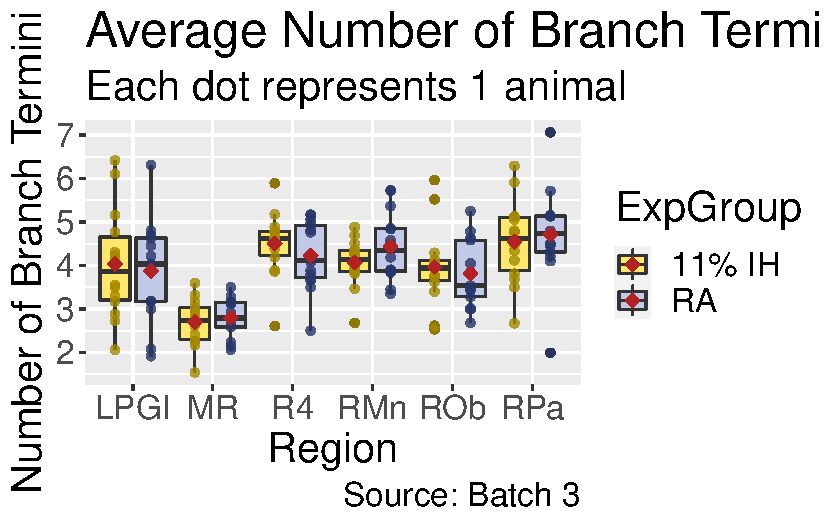
\includegraphics{Fiber_analysis_quarto_files/figure-pdf/fig-expgroup_region-1.pdf}

}

}

\subcaption{\label{fig-expgroup_region-1}}
\end{minipage}%
%
\begin{minipage}[t]{0.33\linewidth}

{\centering 

\raisebox{-\height}{

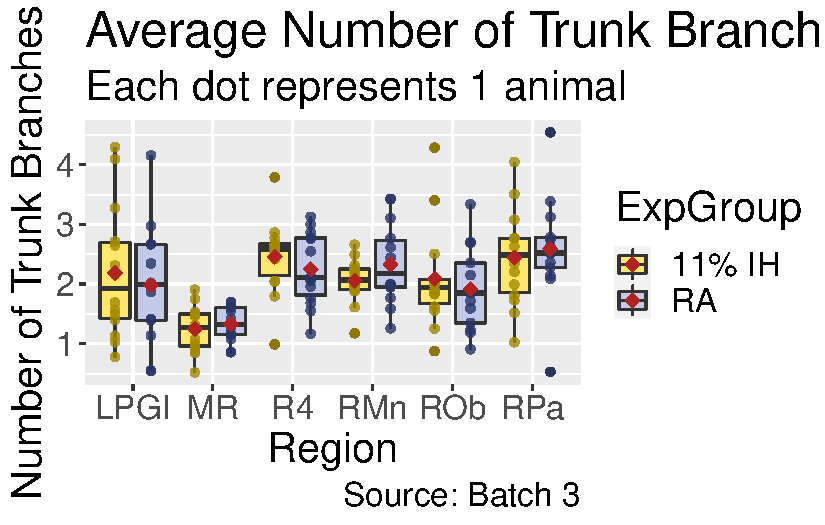
\includegraphics{Fiber_analysis_quarto_files/figure-pdf/fig-expgroup_region-2.pdf}

}

}

\subcaption{\label{fig-expgroup_region-2}}
\end{minipage}%
%
\begin{minipage}[t]{0.33\linewidth}

{\centering 

\raisebox{-\height}{

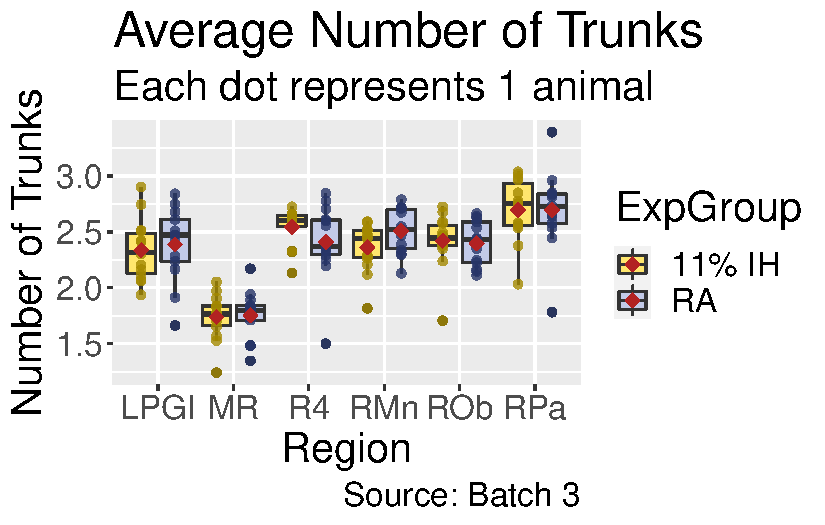
\includegraphics{Fiber_analysis_quarto_files/figure-pdf/fig-expgroup_region-3.pdf}

}

}

\subcaption{\label{fig-expgroup_region-3}}
\end{minipage}%
\newline
\begin{minipage}[t]{0.33\linewidth}

{\centering 

\raisebox{-\height}{

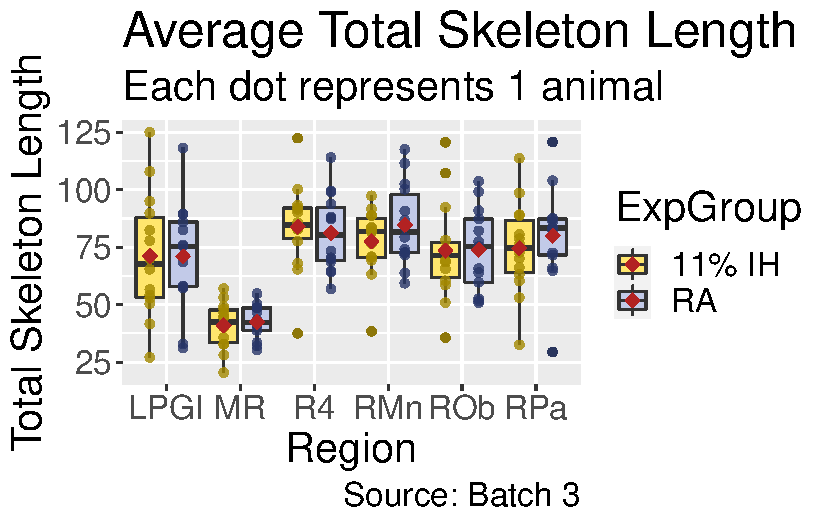
\includegraphics{Fiber_analysis_quarto_files/figure-pdf/fig-expgroup_region-4.pdf}

}

}

\subcaption{\label{fig-expgroup_region-4}}
\end{minipage}%
%
\begin{minipage}[t]{0.33\linewidth}

{\centering 

\raisebox{-\height}{

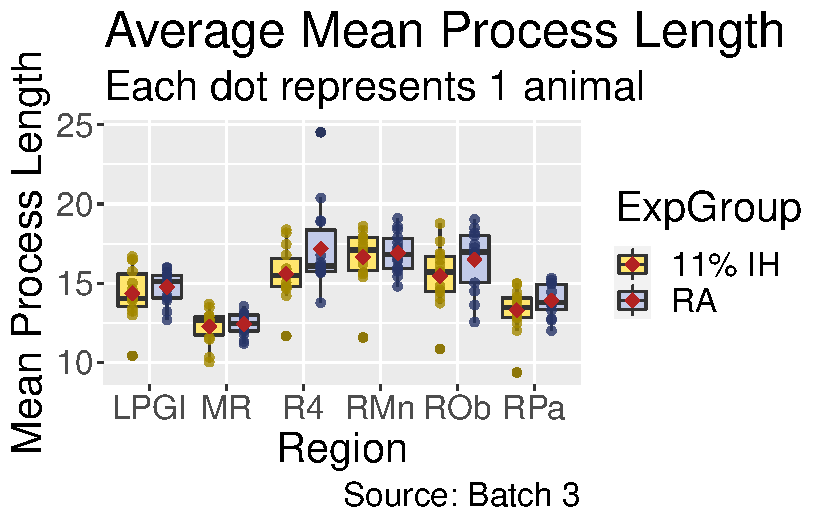
\includegraphics{Fiber_analysis_quarto_files/figure-pdf/fig-expgroup_region-5.pdf}

}

}

\subcaption{\label{fig-expgroup_region-5}}
\end{minipage}%

\caption{\label{fig-expgroup_region}No effect of experimental group on
fiber measures.}

\end{figure}

In examining Mean Process Length, it almost looks like there could be a
difference associated with experimental group in R4. We can look at this
further by conducting a t-test. RA and IH are not statistically
different:

\begin{Shaded}
\begin{Highlighting}[]
\CommentTok{\#t test}
\NormalTok{y\_var}\OtherTok{=}\StringTok{"BorderedCells\_ObjectSkeleton\_avg\_branch\_length"}
\NormalTok{grp1 }\OtherTok{\textless{}{-}}\NormalTok{ region\_df }\SpecialCharTok{\%\textgreater{}\%} \FunctionTok{filter}\NormalTok{(Image\_Metadata\_Region}\SpecialCharTok{==}\StringTok{"R4"}\NormalTok{, ExpGroup}\SpecialCharTok{==}\StringTok{"11\% IH"}\NormalTok{) }\SpecialCharTok{\%\textgreater{}\%} \FunctionTok{pull}\NormalTok{(y\_var)}
\NormalTok{grp2 }\OtherTok{\textless{}{-}}\NormalTok{ region\_df }\SpecialCharTok{\%\textgreater{}\%} \FunctionTok{filter}\NormalTok{(Image\_Metadata\_Region}\SpecialCharTok{==}\StringTok{"R4"}\NormalTok{, ExpGroup}\SpecialCharTok{==}\StringTok{"RA"}\NormalTok{) }\SpecialCharTok{\%\textgreater{}\%} \FunctionTok{pull}\NormalTok{(y\_var)}
\FunctionTok{t.test}\NormalTok{(grp1, grp2)}
\end{Highlighting}
\end{Shaded}

\begin{verbatim}

    Welch Two Sample t-test

data:  grp1 and grp2
t = -1.8325, df = 22.148, p-value = 0.08035
alternative hypothesis: true difference in means is not equal to 0
95 percent confidence interval:
 -3.361794  0.207057
sample estimates:
mean of x mean of y 
 15.60552  17.18289 
\end{verbatim}

Now let's just look overall at RA vs.~IH mice:

\begin{Shaded}
\begin{Highlighting}[]
\NormalTok{p\_list}\OtherTok{=}\FunctionTok{list}\NormalTok{()}
\ControlFlowTok{for}\NormalTok{ (i }\ControlFlowTok{in} \DecValTok{1}\SpecialCharTok{:}\FunctionTok{length}\NormalTok{(measurements)) \{}
\NormalTok{  p\_list[[i]] }\OtherTok{\textless{}{-}} \FunctionTok{plot\_boxwhisker}\NormalTok{(total\_df, measurements, desc, i, }\AttributeTok{x\_var=}\StringTok{"ExpGroup"}\NormalTok{)}
  \FunctionTok{plot}\NormalTok{(p\_list[[i]])}
\NormalTok{\}}

\CommentTok{\#cowplot::plot\_grid(plotlist=p\_list, ncol=2, scale=1)}
\end{Highlighting}
\end{Shaded}

\begin{figure}

\begin{minipage}[t]{0.33\linewidth}

{\centering 

\raisebox{-\height}{

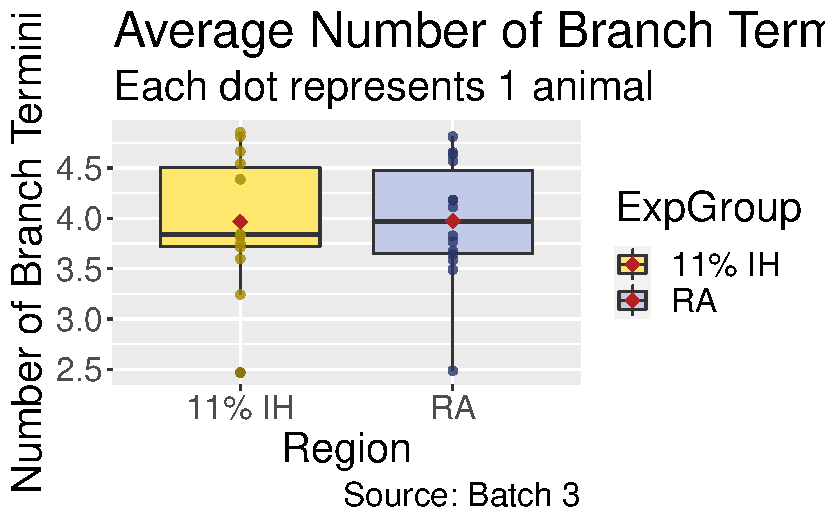
\includegraphics{Fiber_analysis_quarto_files/figure-pdf/fig-expgroup-1.pdf}

}

}

\subcaption{\label{fig-expgroup-1}}
\end{minipage}%
%
\begin{minipage}[t]{0.33\linewidth}

{\centering 

\raisebox{-\height}{

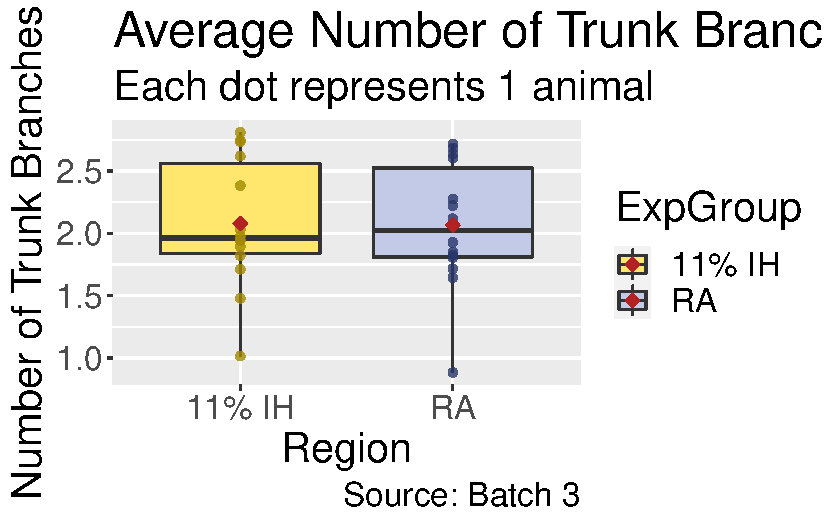
\includegraphics{Fiber_analysis_quarto_files/figure-pdf/fig-expgroup-2.pdf}

}

}

\subcaption{\label{fig-expgroup-2}}
\end{minipage}%
%
\begin{minipage}[t]{0.33\linewidth}

{\centering 

\raisebox{-\height}{

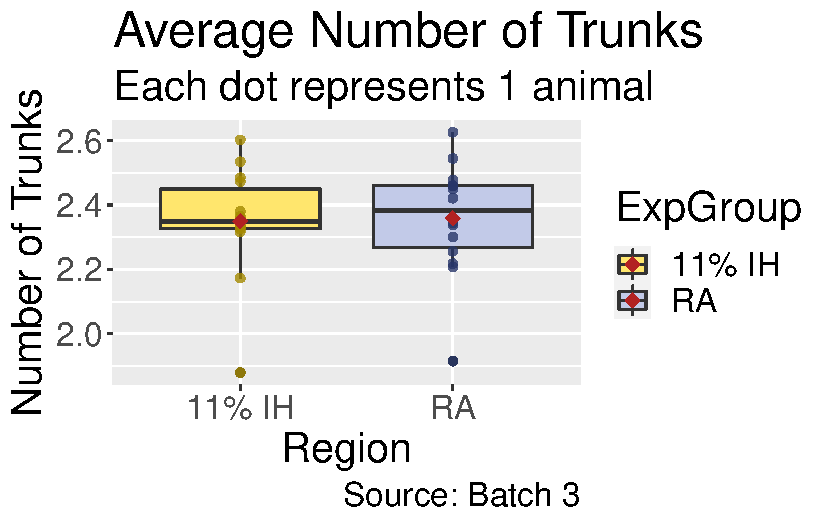
\includegraphics{Fiber_analysis_quarto_files/figure-pdf/fig-expgroup-3.pdf}

}

}

\subcaption{\label{fig-expgroup-3}}
\end{minipage}%
\newline
\begin{minipage}[t]{0.33\linewidth}

{\centering 

\raisebox{-\height}{

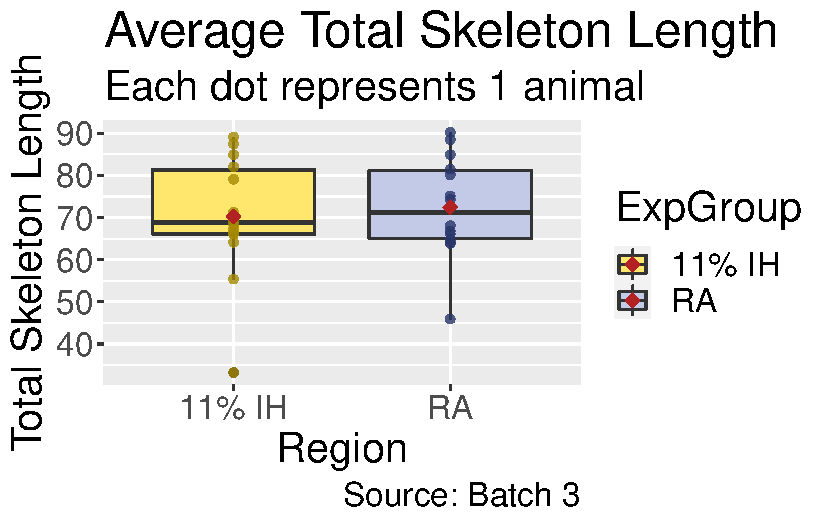
\includegraphics{Fiber_analysis_quarto_files/figure-pdf/fig-expgroup-4.pdf}

}

}

\subcaption{\label{fig-expgroup-4}}
\end{minipage}%
%
\begin{minipage}[t]{0.33\linewidth}

{\centering 

\raisebox{-\height}{

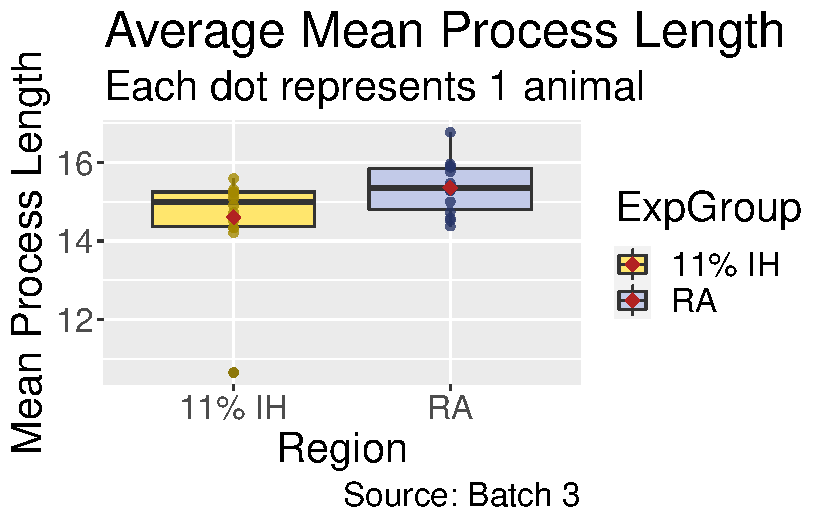
\includegraphics{Fiber_analysis_quarto_files/figure-pdf/fig-expgroup-5.pdf}

}

}

\subcaption{\label{fig-expgroup-5}}
\end{minipage}%

\caption{\label{fig-expgroup}No effect of experimental group on fiber
measures.}

\end{figure}

Instead of viewing each animal as a datapoint, we can also look at the
distribution of all cells. Here's our plotting function:

\begin{Shaded}
\begin{Highlighting}[]
\NormalTok{plot\_distribution }\OtherTok{\textless{}{-}} \ControlFlowTok{function}\NormalTok{(data, measurements, desc, index, x\_var, facetby)\{}
\NormalTok{  p}\OtherTok{\textless{}{-}} \FunctionTok{ggplot}\NormalTok{(sc\_df\_combined, }\FunctionTok{aes}\NormalTok{(}\AttributeTok{x=}\FunctionTok{get}\NormalTok{(measurements[index]), }\AttributeTok{fill=}\NormalTok{ExpGroup, }\AttributeTok{color=}\NormalTok{ExpGroup))}\SpecialCharTok{+}
  \FunctionTok{geom\_density}\NormalTok{(}\AttributeTok{alpha=}\FloatTok{0.7}\NormalTok{, }\AttributeTok{adjust=}\DecValTok{1}\NormalTok{, }\AttributeTok{color=}\ConstantTok{NaN}\NormalTok{)}\SpecialCharTok{+}
  \FunctionTok{scale\_fill\_manual}\NormalTok{(}\AttributeTok{values=}\NormalTok{pal)}\SpecialCharTok{+}
  \FunctionTok{geom\_density}\NormalTok{(}\AttributeTok{alpha=}\FloatTok{0.2}\NormalTok{, }\AttributeTok{adjust=}\DecValTok{1}\NormalTok{, }\AttributeTok{fill=}\ConstantTok{NaN}\NormalTok{)}\SpecialCharTok{+}
  \FunctionTok{scale\_color\_manual}\NormalTok{(}\AttributeTok{values=}\NormalTok{pal\_dark)}\SpecialCharTok{+}
  \FunctionTok{facet\_wrap}\NormalTok{(}\SpecialCharTok{\textasciitilde{}}\FunctionTok{get}\NormalTok{(facetby))}\SpecialCharTok{+}
  \FunctionTok{labs}\NormalTok{(}\AttributeTok{title=}\FunctionTok{paste0}\NormalTok{(}\StringTok{"Distribution of "}\NormalTok{,desc[index], }\StringTok{" by Region, treatment"}\NormalTok{), }
       \AttributeTok{caption=}\StringTok{"Source: Batch 3"}\NormalTok{,}
       \AttributeTok{x=}\NormalTok{desc[index])}\SpecialCharTok{+}
  \FunctionTok{theme\_bw}\NormalTok{()}
  \FunctionTok{print}\NormalTok{(p)}
\NormalTok{\}}
\end{Highlighting}
\end{Shaded}

Let's make some distribution plots:

\begin{Shaded}
\begin{Highlighting}[]
\ControlFlowTok{for}\NormalTok{ (i }\ControlFlowTok{in} \DecValTok{1}\SpecialCharTok{:}\FunctionTok{length}\NormalTok{(measurements)) \{}
  \FunctionTok{plot\_distribution}\NormalTok{(sc\_df\_combined, measurements, desc, i, }\AttributeTok{x\_var=}\StringTok{"ExpGroup"}\NormalTok{, }\AttributeTok{facetby=}\StringTok{"Image\_Metadata\_Region"}\NormalTok{)}
\NormalTok{\}}
\end{Highlighting}
\end{Shaded}

\begin{figure}[H]

{\centering 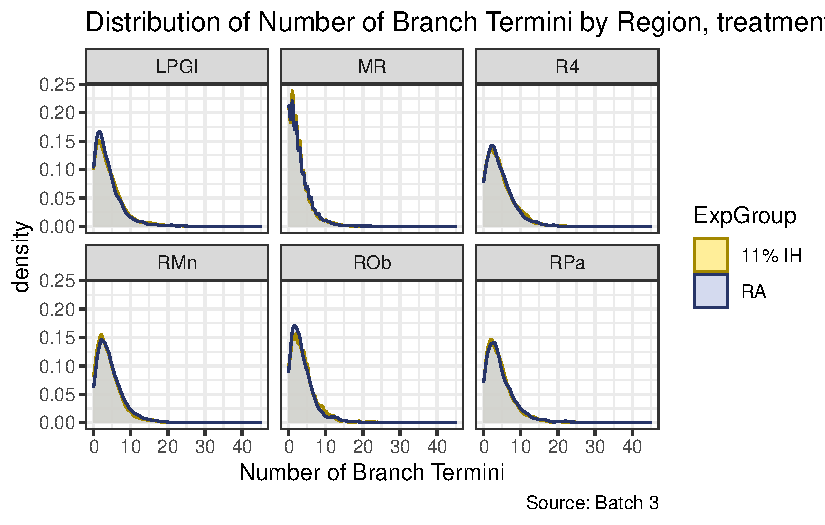
\includegraphics{Fiber_analysis_quarto_files/figure-pdf/make_distribution_plots_region-1.pdf}

}

\end{figure}

\begin{figure}[H]

{\centering 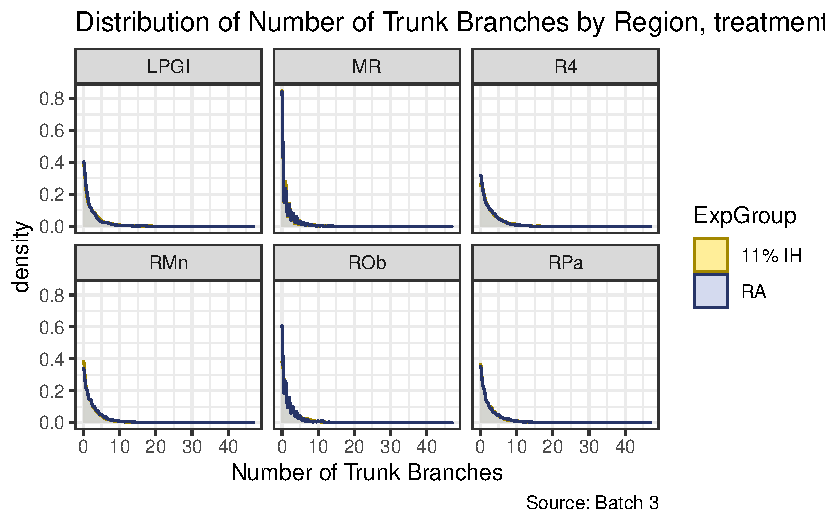
\includegraphics{Fiber_analysis_quarto_files/figure-pdf/make_distribution_plots_region-2.pdf}

}

\end{figure}

\begin{figure}[H]

{\centering 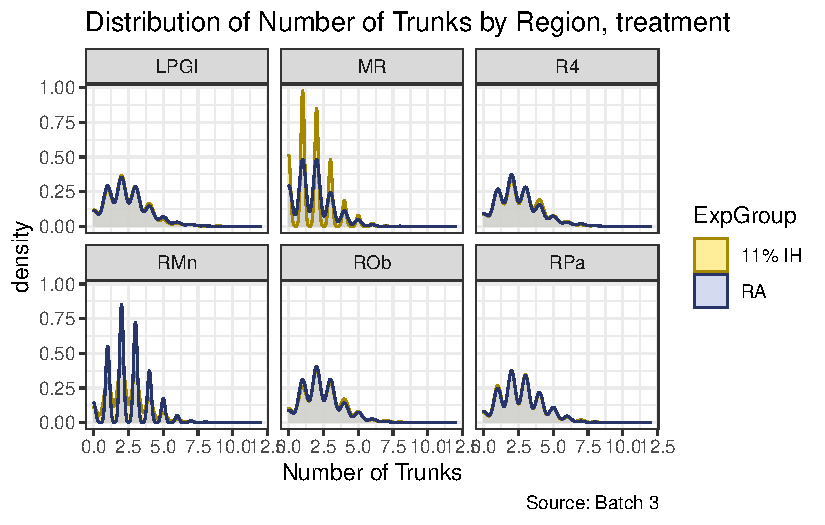
\includegraphics{Fiber_analysis_quarto_files/figure-pdf/make_distribution_plots_region-3.pdf}

}

\end{figure}

\begin{figure}[H]

{\centering 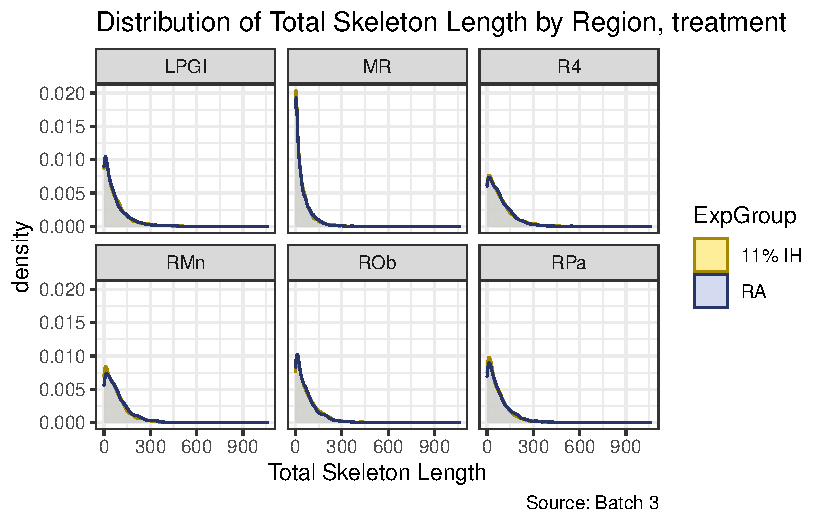
\includegraphics{Fiber_analysis_quarto_files/figure-pdf/make_distribution_plots_region-4.pdf}

}

\end{figure}

\begin{verbatim}
Warning: Removed 2637 rows containing non-finite values (stat_density).
Removed 2637 rows containing non-finite values (stat_density).
\end{verbatim}

\begin{figure}[H]

{\centering 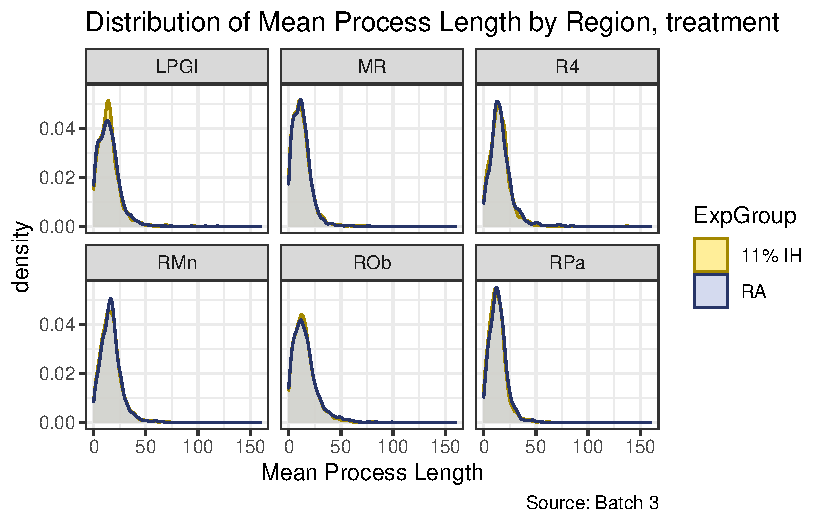
\includegraphics{Fiber_analysis_quarto_files/figure-pdf/make_distribution_plots_region-5.pdf}

}

\end{figure}

\hypertarget{make-summary-table-n-counts-for-mouse-region-treatment}{%
\subsection{Make summary table (n counts for mouse, region,
treatment)}\label{make-summary-table-n-counts-for-mouse-region-treatment}}

\begin{Shaded}
\begin{Highlighting}[]
\NormalTok{tally\_df }\OtherTok{\textless{}{-}}\NormalTok{ sc\_df\_combined }\SpecialCharTok{\%\textgreater{}\%} 
  \FunctionTok{group\_by}\NormalTok{(Image\_Metadata\_Mouse, Image\_Metadata\_Region, ExpGroup, ImageNumber) }\SpecialCharTok{\%\textgreater{}\%}
  \FunctionTok{tally}\NormalTok{(}\AttributeTok{name=}\StringTok{"n\_cells"}\NormalTok{) }\SpecialCharTok{\%\textgreater{}\%} 
  \FunctionTok{select}\NormalTok{(}\SpecialCharTok{{-}}\NormalTok{ImageNumber) }\SpecialCharTok{\%\textgreater{}\%} 
  \FunctionTok{group\_by}\NormalTok{(Image\_Metadata\_Mouse, Image\_Metadata\_Region, ExpGroup) }\SpecialCharTok{\%\textgreater{}\%} 
  \FunctionTok{add\_tally}\NormalTok{(}\AttributeTok{name=}\StringTok{"n\_images"}\NormalTok{) }\SpecialCharTok{\%\textgreater{}\%}
  \FunctionTok{summarize}\NormalTok{(}\AttributeTok{n\_cells=}\FunctionTok{sum}\NormalTok{(n\_cells), }\AttributeTok{n\_images=}\FunctionTok{median}\NormalTok{(n\_images)) }\SpecialCharTok{\%\textgreater{}\%}
  \FunctionTok{mutate}\NormalTok{(}\AttributeTok{n\_cells\_per\_image=}\NormalTok{n\_cells}\SpecialCharTok{/}\NormalTok{n\_images)}
\end{Highlighting}
\end{Shaded}

\begin{verbatim}
`summarise()` has grouped output by 'Image_Metadata_Mouse',
'Image_Metadata_Region'. You can override using the `.groups` argument.
\end{verbatim}

\begin{Shaded}
\begin{Highlighting}[]
\FunctionTok{datatable}\NormalTok{(tally\_df, }
          \AttributeTok{style=}\StringTok{"default"}\NormalTok{,}
          \AttributeTok{rownames=}\ConstantTok{FALSE}\NormalTok{, }
          \AttributeTok{colnames=}\FunctionTok{c}\NormalTok{(}\StringTok{"Mouse"}\NormalTok{, }\StringTok{"Region"}\NormalTok{, }\StringTok{"Group"}\NormalTok{, }\StringTok{"n cells"}\NormalTok{, }\StringTok{"n images"}\NormalTok{, }\StringTok{"n cells per image"}\NormalTok{),}
          \AttributeTok{extensions =} \StringTok{\textquotesingle{}Buttons\textquotesingle{}}\NormalTok{,}
          \AttributeTok{fillContainer =} \ConstantTok{FALSE}\NormalTok{,}
          \AttributeTok{options =} \FunctionTok{list}\NormalTok{(}
            \AttributeTok{pageLength =} \DecValTok{20}\NormalTok{, }
            \AttributeTok{dom =} \StringTok{\textquotesingle{}Bfrtip\textquotesingle{}}\NormalTok{,}
            \AttributeTok{buttons =} \FunctionTok{c}\NormalTok{(}\StringTok{\textquotesingle{}copy\textquotesingle{}}\NormalTok{, }\StringTok{\textquotesingle{}print\textquotesingle{}}\NormalTok{, }\StringTok{\textquotesingle{}csv\textquotesingle{}}\NormalTok{, }\StringTok{\textquotesingle{}excel\textquotesingle{}}\NormalTok{, }\StringTok{\textquotesingle{}pdf\textquotesingle{}}\NormalTok{)}
\NormalTok{            )}
\NormalTok{          )}
\end{Highlighting}
\end{Shaded}

\begin{Shaded}
\begin{Highlighting}[]
\CommentTok{\#total\_count\_RA \textless{}{-} sc\_df\_combined \%\textgreater{}\% filter(ExpGroup=="RA") \%\textgreater{}\% count() \%\textgreater{}\% pull()}
\CommentTok{\#total\_count\_IH \textless{}{-} sc\_df\_combined \%\textgreater{}\% filter(ExpGroup=="11\% IH") \%\textgreater{}\% count() \%\textgreater{}\% pull()}
\end{Highlighting}
\end{Shaded}




\end{document}
